\documentclass[11pt]{article}

\usepackage{float}
\usepackage[T1]{fontenc}
\usepackage[left=12mm,
right=12mm,top=1.0in,
bottom=1.5in]{geometry}
\usepackage{amsmath}
\usepackage{mathtools}
\usepackage{cancel}
\usepackage{graphicx}
\usepackage{grffile}
\usepackage{caption}
\setcounter{section}{-1}
\graphicspath{{/home/piotr/Documents/scientific-computing/list05/plots/}}
\DeclareUnicodeCharacter{2212}{-}

\begin{document}
\title{{Obliczenia Naukowe}}
\author{Laboratorium Lista Nr 5\\Piotr Popis\\ 245162}
\date{6 grudzień 2019}
\maketitle
\centering

\begin{flushleft}
\section{Wstęp}
\subsection{Streszczenie}
Problemem jest rozwiązanie równania liniowego $Ax=b$,gdzie $A \epsilon R^{nxn}$ jest podaną macierzą, a $b \epsilon R^n$ zadanym wektorem prawych stron( przy założeniu, iż $n \geq 4$ ).
Dodatkowo macierz A jest macierzą rzadką- taką, która ma dużo elementów zerowych oraz blokową.
\[
A=\begin{bmatrix}
      A_1 & C_1 & 0 & ... & 0 \\
    B_2 & A_2 & C_2 & .. & 0 \\
    \vdots & \ddots & \ddots & \ddots & \vdots \\
     0 & ... & B_{v-1} & A_{v-1} & C_{v-1} \\
      0 & ... & 0 & B_v & A_v \\
  \end{bmatrix}
\]
, gdzie $v=\dfrac{n}{l}$ przy założeniu iż l zawsze dzieli n( n jest podzielne przez l) oraz $l\geq2$. l jest rozmiarem wszystkich kwadratowych macierzy wewnętrznych - bloków: $A_k, B_k, C_k$. Mianowicie: $$A_k \epsilon R^{lxl}, k = 1,...,v  ,$$ A jest macierzą gęstą, \\0 jest kwadratową macierzą zerową stopnia l,\\Natomiast macierz $$B_k \epsilon R^{lxl}, k = 2,...,v  ,$$ $B_k$ ma tylko \underline{dwie ostatnie kolumny niezerowe} i jest postaci:   
\[
B_k=\begin{bmatrix}
      0 & ... & 0 & b^k_{1l-1} & b^k_{1l} \\
      0 & ... & 0 & b^k_{2l-1} & b^k_{2l} \\
      \vdots &     & \vdots & \vdots & \vdots \\
      0 & ... & 0 & b^k_{ll-1} & b^k_{ll} \\
  \end{bmatrix}
\]
Ostani z bloków $$C_k \epsilon R^{lxl}, k = 1,...,v-1  ,$$ $C_k$ jest macierzą diagonalną i jest postaci:
\[
C_k=\begin{bmatrix}
      c^k_1 & 0 & 0 & ... & 0 \\
    0 & c^k_2 & 0 & .. & 0 \\
    \vdots & \ddots & \ddots & \ddots & \vdots \\
     0 & ... & 0 & c^k_{l-1} & 0 \\
      0 & ... & 0 & 0 & c^k_l \\
  \end{bmatrix}
\]
Z treści n jest ogromne co wiąże się dużym obciążeniem pamięciowym jak i czasowym w przypadku zwykłej tablicy. Należy skorzystać z pakietu SparseArrays, która zawiera specjalną strukturę efektywnie pamiętająca specyficznie macierze, tj rzadkość lub regularność występowania elementów zerowych i niezerowych. Istniejące algorytmy do rozwiązywania takich problemów trzeba po prostu zmodyfikować do użycia tej spejcalnej struktury. Jeśli l jest stałe Algorytmy da się zoptymalizować czasowo z $\mathcal{O}(n^3)$ do  $\mathcal{O}(n)$.\\
\subsection{Treść}
\paragraph{Zadanie 1} Należy stworzyć funkcję rozwiązującą układ $Ax=b$ metodą eliminacji Gaussa uwzględniającą postać macierzy A zadanej w streszczeniu dla dwóch wariantów \\ (a)bez wyboru elementu głównego \\(b)z częściowym wyborem elementu głównego\\ \paragraph{Zadanie 2} Należy napisać funkcję wyznaczającą rozkład $LU$ macierzy A metodą eliminacji Gauss'a uwzględniającą specyficzną postać macierzy $A$ dla \\ (a)bez wyboru elementu głównego \\(b)z częściowym wyborem elementu głównego \\ \paragraph{Zadanie 3} Należy napisać funkcję rozwiązującą układ równań $Ax=b$ ( uwzgledniającą specyficzną postać macierzy $A$ ).\\
\bigskip
Wszystkie funkcje powinny byc umieszczone w module o nazwie blocksys. Należy przeczytać Sparse Arrays manual Julia. Założyć, że dostęp do elementu macierzy jest w czasie stałym. Nie można używać $x=\dfrac{A}{b}$ oraz $lu$ z modułu LinearAlgebra.
\section{Zadanie 1}
\subsection{Opis standardowej procedury wraz z analizą złożoności algorytmu}
\paragraph{Na czym polega metoda eliminacji Gauss'a?}
Metoda ta polega na sprowadzeniu układu równań( macierzy) do równoważnego układu z wykorzystaniem macierzy trójkątnej górnej,  następnie rozwiązaniu tego układu przy pomocy algorytmu podstawiania wstecz.
\paragraph{Na czym polega algorytm podstawiania wstecz?}
Algorytm ten bazuje na zerowaniu kolejnych elementów macierzy poniżej diagonali( czyli tej niezerowej przekątnej).
\paragraph{Przebieg procedury}  1. Zerowanie elementów poniżej pierwszego wiersza w pierwszej kolumnie.\\2. Ogólnie, aby wyzerować $a_{i1}$ od wiersza i-tego odejmowany jest wyraz pierwszy pomnżony przez liczbę $\dfrac{a_{i1}}{a_{11}}$ \\ 3. Następnie przechodzimy do kolejnej kolumny( tutaj drugiej itd) i powtarzamy powyższe procedury z taką zmianą, że teraz odejmowany wiersz i( tutaj drugi $a_{22}$ itd).\\
Niestety procedura nie zadziała jeśli którtkolwiek z diagonalnych elementów będzie zerem( jak widać we wzorze). Aby rozwiązać ten problem należy przeprowadzić odpowiednią modyfikację. W i-tym kroku , w i-tej kolumnie należy wyszukać w kolejnych wierszach j-ty element o wartości co do modułu największej i zamienić wtedy $a_{ii}$ z $ a_{ji}$ (wzór: $a_{wierszkolumna}$).\\Następnie korzystamy z algorytmu wstecz, czyli matematycznie wzoru: $x_i = \dfrac{b_i-\sum^n_{j=i+1} a_{ij}}{a_{ii}}$.\\ 
Począwszy od ostatniego indeksu.( n)\\
Zakładając, że n jest rozmiarem macierzy złożonośc obliczeniowa eliminacji Gaussa wynosi co najwyżej $\mathcal{O}(n^3)$, a algorytm podstawiania wstecz $\mathcal{O}(n^2)$. Łącznie, aby rowiązać układ należy wykonać $\mathcal{O}(n^3)$ operacji.
\subsection{Opis implementacji wraz z analizą złożoności algorytmu}
\subsubsection{SparseMatrix pamięć}
Celem zadania jest modyfikacja i optymalizacja algorytmu. Zauważmy, że rozpatrywana macierz ma dość specyficzną, nietypową postać. Jest macierzą rzadką. Ma $(l+3)n-3l$ elementów, które nie są zerami.\\
\begin{center}
$l^2$ - w każdym z v bloków $A_k$, \\ $2l$ - w każdym z v-1 bloków $B_k$, \\ $l$ - w każdym z v-1 bloków $C_k$\end{center} Do przechowywania macierzy wykorzystamy struktuę do przechowywania macierzy rzadkich SparseMatrixCSC. Macierze takie są przechowywane w skompresowanym porządku kolumnowym. Algorytm Gauss'a natomiast ma przebieg wierszowy, zatem w implementacji musimy zamienić miejscami indeksy kolumny i wiersza i pracować na macierzach trasnponowanych. Aby ułatwić proces zrozumienia algorytmu uznaję to za problem implementacyjny i indeksuję w roważaniach w sposób standardowy. \underline{Dzięku użyciu takiej struktury mamy szybszy dostęp do elementów.}
\subsubsection{Modyfikacja, optymalizacja algorytmu}
Zwrócmy uwagę na postać macierzy A. Jest to macierz diagonalna, a nawet trójdiagonalna. W dodatku jest to macierz blokowa( $A_k,B_k,C_k$). Zauważmy, że nie jest konieczne zerowanie wszystkich elementów poniżej diagonali( przekątnej), bo już są wyzerowane. \\ \underline{Pozwala to zredukować ilość wykonywanych obliczeń.}\\ 
\paragraph{Indeks rzędu ostatniego niezerowego elementu w kolumnie} W pierwszych $l-2$ kolumnach potencjalne niezerowe elementy znajdują sie w $l$-pierwszych rzędach i są to elementy bloku $A_1$, dla kolejnych $l$ kolumn elementy niezerowe znajdują się prawdopodobnie w pierwszych $2l$ rzędach są to elementy bloku $A_3$ oraz dwie ostatnie kolumny bloku $B_2$. W kolejnych l kolumnach niezerowe elementy znajdują się w peirwszych 3l rzędach są nimi elementy bloku $B_3$ oraz elementy bloku $A_4$ rzecz jasna niezerowe elementy.\\
Zatem ostatni niezerowy element w danej kolumnie można obliczyć korzystając z funkcji min(). Ostatecznie ostatni niezerowy element w kolumnie wyrażamy wzorem: $ lastNotZeroInColumn(column) = min \Big( n,$ $l+l \Big \lfloor \dfrac{column+1}{l} \Big \rfloor \Big)$
\paragraph{Indeks kolumny ostatniego niezerowego elementu w rzędzie} 
Zwróćmy teraz uwagę na wiersze. W każdym wierszu ostatnim elementem niezerowmy jest element diagonali bloku $C$. Poza pierwszym wierszem, każdy z tych elementów jest oddalony równo o $l$ od elementów całej macierzy. W ostatnich rzędach ostatnie niezerowe elementy to po prostu elementy ostatniego bloku $A_v$ leżące pod indeksem $n$. \\Ostatecznie ostatni niezerowy element w rzędzie to:
$$lastNotZeroInRow(row) = min(n, row+l)$$ \\
Znając indeksy ostatniego niezerwowego elementu w rzędzie i kolumnie wiemy, do jakiego miejsca jest sens wykonywać obliczenia. Pozwala to znacznie przyspieszyć proces obliczania.\\
Metoda eliminacji Gauss'a doprowadza nas do macierzy trójkątnej górnej, który rowiązujemy przy pomocy algorytmu podstawiania wstecz. Mimo dotychczasowych usprawnień zauważyłem również, że wciąż algorytm można usprawnić. Algorytm eliminacji Gaussa przecież nie dostawia elementów niezerowych do danej macierzy( Poza elementami pod diagonalą bloków C). Zatem można skorzystać z wzoru na  $lastNotZeroInRow$ i sumować elementy tylko do określonego indeksu.
\subsubsection{Analiza złożoności obliczeniowej zmodyfikowanego algorytmu}
Zakładam, że l jest stałą. \\
Zewnętrzna pętla i eliminacji Gauss'a  wykonuje n-1 przejść, wewnętrzna j wykonuje dokładnie 2l przebiegów, a najbardziej wewnętrzna k i nie mająca w sobie żadnego innego zagnieżdżenia l opracji. Zewnętrzna pętla podstawiania wykonuje n przejść, a wewnętrzna co najwyżej l. W sumie łącznie dla eliminacji mamy $2l^2n$ operacji, a dla podstawiania $nl$, zatem złożoność wynosi $\mathcal{O}(n)$ nazywana złożonością liniową.
\subsection{Algorytm z częściowym wyborem elementu głownego rozwiązanie problemu zerowego elementu diagonali}
Jak już wspomnieliśmy w paragrafie \textsl{Przebieg procedury} na początku sekcji \textsl{2.1 Opis standardowej procedury wraz z analizą złożoności algorytmu} możemy napotkać na sytuację, w której nasz algorytm nie zadziała. Mianowicie, gdy którykolwiek z elementów diagonali będzie zerem. Na szczęście problem ten można rozwiązać w dość prosty sposób rozwiązać. W każdej kolumnie przed rozpoczęciem zerowania wybrać maksymalny co do wartości bezwzględnej element w kolumnie i uznać go za element, od którego będziemy odejmować.
\paragraph{Jak wyglądają modyfikacje wynikające z częściowego wyboru elementu głownego?}
Zacznijmy od analizy kolumny. Samo ograniczenie ostatniego, maksymalnego niezerowego argumentu w danej kolumie się nie zmieni, natomiast wartość podlega wątpliwości. W wyniku zamiany rzędami argumentu leżacego wyżej z leżącym niżej i kolejnym odejmowaniu go od wierszy poniższych możemy napotkać się na sytuację, w której program wypełni zerowy argument. Granicznym przypadkiem jest oczywiście zamiana i-tego wiersza z wierszem ostatnim( niezerowym),zatem wzór na ostatni niezerwoy element w danej kolumnie należy zmienić, tzn: $$ lastNonZeroInRow(lastNonZeroInColumn(row))= min(lastNonZeroInColumn(row)+l,n) =
$$
$$ = min(min \Big( n, l+l \Big \lfloor \dfrac{row+1}{l} \Big \rfloor \Big) +l,n) = min \Big( n, \underline{2l}+l \Big \lfloor \dfrac{row+1}{l} \Big \rfloor \Big) $$
Ostatecznie teraz indeks kolumny ostatniego niezerowego elementu w wierszu wyznaczamy wzorem : $$min \Big( n, \underline{2l}+l \Big \lfloor \dfrac{row+1}{l} \Big \rfloor \Big)$$ można je uznać za górne ograniczenie, czyli max indeks kolumny w row-wym wierszy \textsl{po przepermutowaniu}.
W celu uniknięcia nadużycia zasobów pamięci wykorzystam addytywną tablicę permutacji, zawierjącą indeksy kolejnych wierszy macierz. Zamiana zatem wykonywana jest na kopii, polega na odwołaniu się do tablicy permutacji np pod indeksem row będzie leżał row-ty wiersz z macierzy. 
\subsection{Analiza złożoności obliczeniowej zmodyfikowanego algorytmu z częściowym wyborem elementu głownego}
Wariant ten jest nieco bardziej kosztowany. Pojawia się koszt wyszukania maksymalnego elementu głownego o największej co do wartości bezwzględnej wartości w danej "zerowanej", bieżącej kolumnie. Wyszukanie go występuje w $lastNotZeroInColumn - i$ elementów, w przybliżeniu uznaję za $2l$.Wewnętrzna pętla przechodzi po $3l$ elementów każdego z wierszy. Ostatecznie koszt to $n2l(2l+3l)=10l^2n$, zatem jest około 5 razy bardziej złożony obliczeniowo niż algorytm bez wyboru elementu głownego. Mimo to algorytm jest wciąż asymptotycznie liniowy $
\mathcal{O}(n)$
\section{Zadanie 2}
\subsection{Opis standardowej procedury wraz z analizą złożoności algorytmu}
\paragraph{Na czym polega rozkład LU} Rozkład LU polega na takim rozłożeniu macierzy A na czynniki L oraz U, gdzie obydwie macierze są macierzami trójkątnymi z tym, że U jest macierzą trójkątną górną, a L jest macierzą trójkątną dolną. Inaczej mówiąc rozkład LU polega na przedstawieniu macierzy A w potaci iloczynu $$A = LU$$ z zadanymi warunkami. Dodatkowo zakładamy, że wszystkie elementy diagonalne macierzy $L$ są równe 1.\\ 
\subsection{Opis implementacji wraz z analizą złożoności algorytmu}
Algorytm wyznaczania rozkładu $LU$ przebiega sposób identyczny jak algorytm eliminacji Gauss'a z punktu $1.2$ z jedną modyfikacją. Mianowicie w miejscach, w których wcześniej zapisywaliśmy zera poniżej otrzymanej macierzy górnej trójkątnej teraz będziemy zapisywać ilorazy $z = \dfrac{a_{ij}}{a_{jj}} $. Następnie wykorzystamy je jako elementy macierzy $L$, a pozostałe zostaną elementami macierzy $U$. Oczywiście w przypadku samego rozkładu nie używamy algorytmu wstecz, ale nie wpływa to na złożoność, która wciąż jest liniowa. Złożoność w takim wypadku jest taka sama jak dla zmodyfikowanego algorytmu eliminacji Gauss'a, czyli $\mathcal{O}(n)$.
\subsection{Algorytm z częściowym wyborem elementu głownego}
Algorytm wyznaczania rozkładu $LU$ przebiega sposób identyczny jak algorytm eliminacji Gauss'a z punktu $1.3$ z wyborem częściowym elementu głownego także z modyfkiacją, iż w miejsce zerowanych elementów wstawiamy ilorazy $z = \dfrac{a_{ij}}{a_{jj}} $ oraz faktem, iż metoda ta zwróci wektor permutacji $p$ potrzebny do przywrócenia początkowego porządku wierszy w macierzy. Nie używamy algorytmu wstecz do wyznacznenia rozkładu, ale nie zmienia to naszej złożoności. Złożoność w tym przypadku tak jak w powyższym jest analogiczna i liniowa, czyli wynosi  $\mathcal{O}(n)$.
\section{Zadanie 3}
\subsection{Rozwiązywanie układu równań przy użyciu rozkładu LU}
Rozkład LU możemy otrzymać w wyniku przeprowadzenia elimiacji Gauss'a. Czynnik $U$ uzyskujemy w wyniki przekształcenia macierzy $A$ w skutek użycia wyżej wymienionego algorytmu. Natomiast macierz $L$ możemy stworzyć wykorzystując czynniki $z$ użyte do zerowania macierzy. Wtedy zapisujemy mnożnik użyty w i-tym wierszu , w j-tej kolumnie w odpowiadającej jej komórce macierzy $L$. Do przeprowadzenia rozkładu musimy wykonać $\mathcal{O}(n^3)$ działań. Wykorzystanie rozkładu LU jest jednak zdecydowanie skuteczniejsze jeśli zamierzamy użyć tej samej macierzy przy wielu układach, wtedy algorytm eliminacji Gauss'a wykonany jest raz. A następnie układu dzielimy na dwa etapy:
$$
\left\{ 
\begin{array}{ll}
Lz = b\\
Ux = z\\
\end{array} \right.
$$
Koszt zostaje zredukowany do $\mathcal{O}(n^2)$. Tak więc rozwiązanie układu równań w sytuacji, kiedy mamy rozkład LU to rozwiązanie dwóch równań z macierzą trójkątną dolną oraz górną.\paragraph{Jak to osiągnąć?} Należy wykorzystać w odpowdni sposób znane już nam algorytmy podstawiania w przód i wstecz poznane już na pierwszej liście. Struktura naszych macirzy w obu przypadkach pozwala zredukować ilość wykonywanych operacji. \paragraph{Jak teraz będą wyglądać nasze ogranicznia?} Dla algorytmu podstawiania wstecz ograniczenie już wyznaczliśmy. Indeks ostatniej niezerowej kolumny w danym wierszu bez wyboru elementu głównego wyraża się wzorem $lastNotZeroInRow(row) = min(n, row+l)$, \\natomiast z wyborem częściowym elementu głownego wzoru $lastNotZeroInRow(row) = min \Big( n, \underline{2l}+l \Big \lfloor \dfrac{row+1}{l} \Big \rfloor \Big) $.  Pojawia się więc konieczność wyznaczenia wzoru dla algorytmu podstawiania w przód. Pierwszy niezerowy indeks kolumny to $firstNotZeroInRow = min \Big( n, l \Big \lfloor \dfrac{row-1}{l} \Big \rfloor \Big)$.
\subsection{Analiza złożoności}
W kazdym kolejnym wierszu wykonywane jest wykonane $\mathcal{O}(l)$ operacji. Wierszy jest n. Ostatecznie , gdy dany jest rozkład LU  macierzy rowiązanie układu równań wymaga wykonanaie $nl$, zatem $\mathcal{O}(n)$ operacji. 
\newpage
\section{Wyniki eksperymentów porównujących zaimplementowane algorytmy dla danych testowych( tabele, wykresy) oraz interpretacja}
Do sprawdzenia poprawności zaimplementowanych metod utworzono funkcję computeRSV, która generuje takie wektory prawych stron, aby rowiązaniem układu był wektor $(1,...,1)^T$. Następnie przy użyciu zaimplementowanych funkcji rowiązano układy $Ax=b$. Policzono czasy oraz błędy względne umieszczone wyniki poniżej.
\subsection{Porównanie błędów względnych}
\begin{tabular}{|l|l|l|l|l|}
 \hline
  n & Gauss & GaussWithPivot & LU & LUWithPivot\\
 \hline

\hline
 1000 & 2.933079611128323e-14  & 1.0677494543754276e-15  & 2.9268827938365774e-14 & 9.009512859023695e-16 \\
\hline
 5000 & 1.6706355850088109e-13  & 1.8192223023676713e-15  & 3.234648622831034e-13 & 9.052246850857828e-16 \\
\hline
 10000 & 3.6738202190459565e-14  & 7.359706866734175e-16  & 3.6304377614821076e-14 & 4.46959574538234e-16 \\
\hline
 25000 & 8.714734067251055e-14  & 1.3797382568317616e-15  & 8.666083060971685e-14 & 9.326906914352039e-16 \\
\hline
\end{tabular}
\subsection{Porównanie złożoności czasowych}
\begin{tabular}{|l|l|l|l|l|l|}
 \hline
  n & Gauss & GaussWithPivot & LU & LUWithPivot \\
 \hline

\hline
 1000 & 0.001832316  &  0.002586071 & 0.002002504  & 0.007397194  \\
\hline
 5000 &   0.028314322 & 0.030649873  &  0.028153167 & 0.087562782  \\
\hline
 10000 & 0.127289973 & 0.143771038  & 0.129024203 & 0.369629081   \\
\hline
 25000 &  1.122852877 &  0.923107817  & 1.247497774 & 1.10793138   \\
\hline
\end{tabular}
\subsection{Porównanie złożoności pamięciowych}
\begin{tabular}{|l|l|l|l|l|l|}
 \hline
  n & Gauss & GaussWithPivot & LU & LUWithPivot & (A, b) \\
 \hline

\hline
 1000 & 0.1143798828125  &  0.12213134765625 & 0.12213134765625  & 0.1298828125 & 1.5226058959960938\\
\hline
 5000 &   0.5720977783203125 & 0.610321044921875  &  0.610321044921875 & 0.6485443115234375 & 7.540489196777344 \\
\hline
 10000 & 1.1443023681640625 & 1.220672607421875  & 1.220672607421875 & 1.2970428466796875 & 15.063072204589844\\
\hline
 25000 &  2.8609161376953125 &  3.051727294921875  & 3.051727294921875 & 3.2425384521484375  & 37.630821228027344\\
\hline
\end{tabular}
\subsection{Wykresy}
\begin{figure}[H]
\centering
  \begin{minipage}[b]{.45\textwidth}
    \centering
    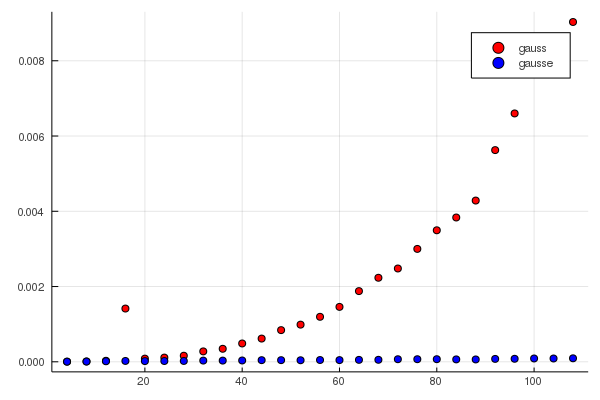
\includegraphics[width=.8\linewidth]{stand_time_size.png}
    \caption{Porównanie złożoności czasowej dla GaussianElimination standardowej i zmodyfkiowanej.}
  \end{minipage}
\end{figure}
\centering
\begin{figure}[]
  \begin{minipage}[b]{.45\textwidth}
    \centering
    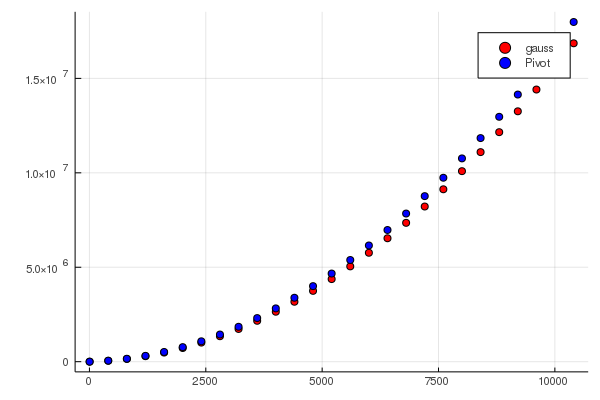
\includegraphics[width=.8\linewidth]{gauss_memory_size.png}
    \caption{Porównanie złożoności pamięciowej dla GaussianElimination z i bez pivot.}
  \end{minipage}\hfill
  \begin{minipage}[b]{.45\textwidth}
    \centering
    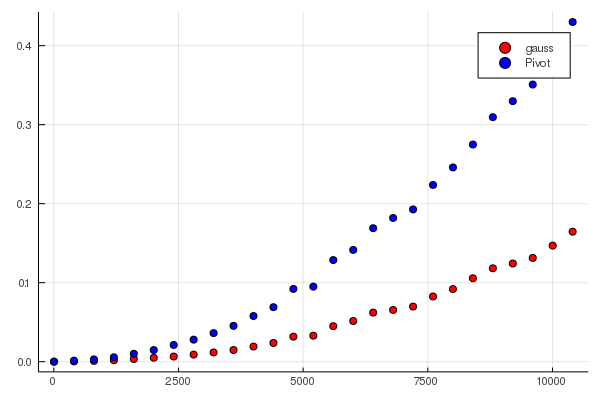
\includegraphics[width=.8\linewidth]{gauss_time_size.png}
    \caption{Porównanie złożoności czasowej dla GaussianElimination z i bez pivot}
  \end{minipage}
  \begin{minipage}[b]{.45\textwidth}
    \centering
    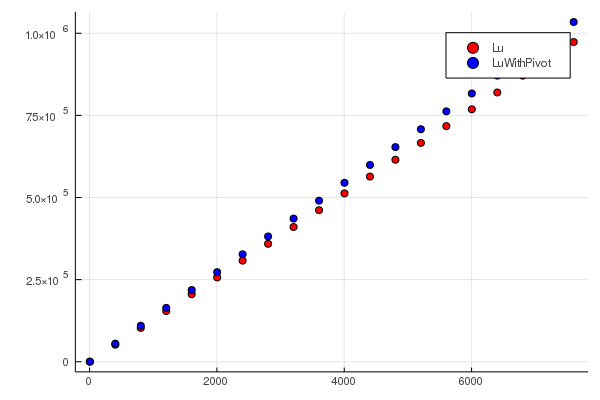
\includegraphics[width=.8\linewidth]{LU_memory_size.png}
    \caption{Porównanie złożoności pamięciowej dla  LU z i bez pivot.}
  \end{minipage}\hfill
  \begin{minipage}[b]{.45\textwidth}
    \centering
    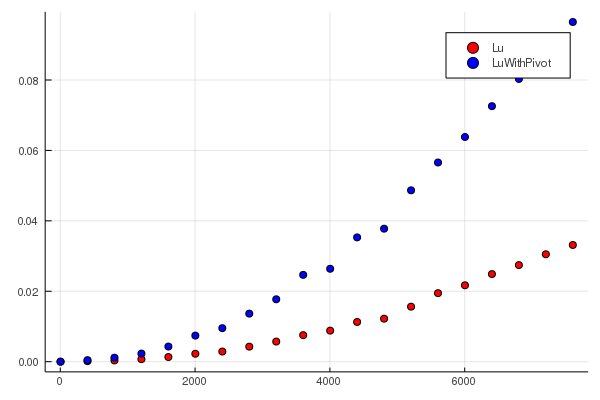
\includegraphics[width=.8\linewidth]{LU_time_size.png}
    \caption{Porównanie złożoności czasowej dla  LU z i bez pivot.}
  \end{minipage}
  \begin{minipage}[b]{.45\textwidth}
    \centering
    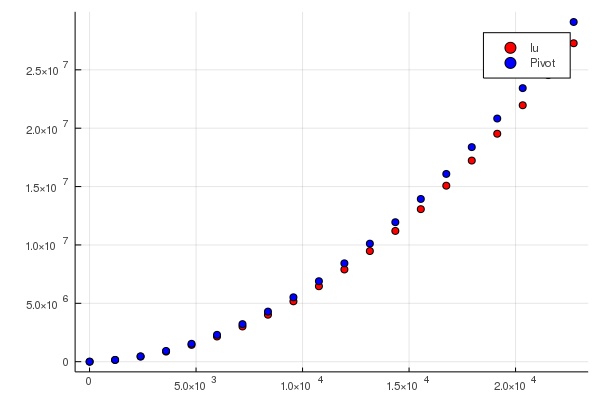
\includegraphics[width=.8\linewidth]{GAUSSxLU_memory_size.png}
    \caption{Porównanie złożoności pamięciowej dla GaussianElimination i LU.}
  \end{minipage}\hfill
  \begin{minipage}[b]{.45\textwidth}
    \centering
    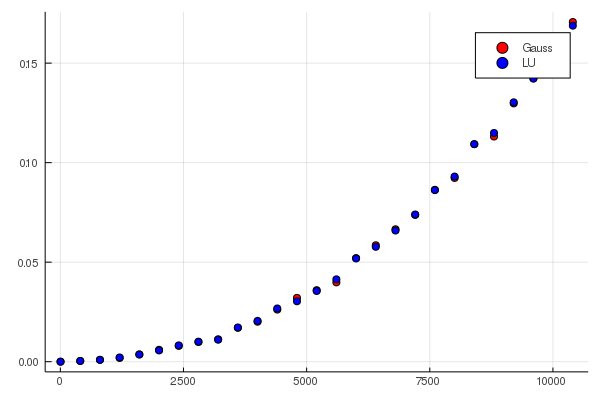
\includegraphics[width=.8\linewidth]{GAUSSxLU_time_size.png}
    \caption{Porównanie złożoności czasowej dla GaussianElimination i LU.}
  \end{minipage}
  \end{figure}
\begin{figure}[H]
    \begin{minipage}[b]{.45\textwidth}
    \centering
    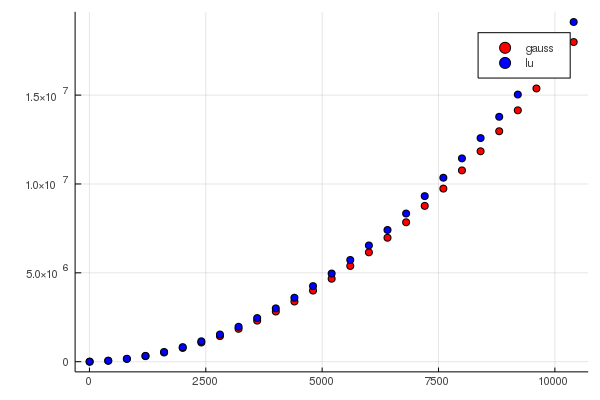
\includegraphics[width=.8\linewidth]{GAUSSxLUpivoted_memory_size.png}
    \caption{Porównanie złożoności pamięciowej dla GaussianElimination i LU z pivot.}
  \end{minipage}\hfill
  \begin{minipage}[b]{.45\textwidth}
    \centering
    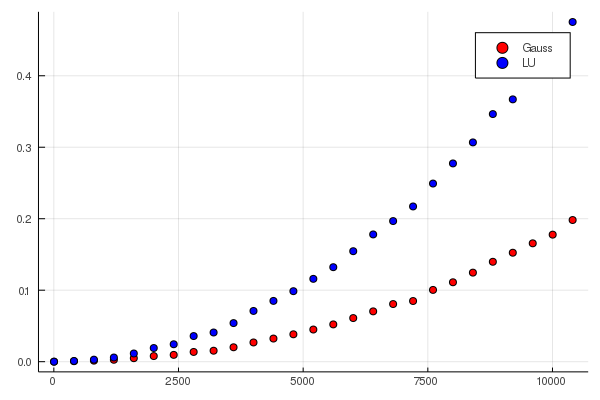
\includegraphics[width=.8\linewidth]{GAUSSxLUpivoted_time_size.png}
    \caption{Porównanie złożoności czasowej dla GaussianElimination i LU z pivot.}
  \end{minipage}
\end{figure}
\newpage
\begin{flushleft}
\section{Wnioski}

\end{flushleft}
\end{flushleft}
\end{document}